\section{Discussion and Future Work}
\label{sec:discussion}

% Summarize, restate contributions.
In this paper, we present a probabilistic approach to automatically coloring 2D patterns. We develop a factor graph model that is trained on example pattern colorings to statistically capture their coloring style and sampled using MCMC to generate a variety of pattern coloring suggestions. We demonstrate the utility of the model on a range of coloring tasks, and a perceptual study showed that the colorings it generates compare favorably to those generated by other automatic methods.

% Frame the discussion
There is still much work to be done to understand what makes a pattern coloring good. In this paper, we propose modeling one plausible set of color properties, and we gain some insight into which properties matter most by comparing their automatically-tuned weights. While colorings generated by the resulting model are attractive and useful, our evaluation shows that they do not yet achieve the same quality as colorings created by human artists. More research is needed to close this gap, and our probabilistic framework provides a strong and flexible foundation for further investigation.

% Discuss limitations, etc.
One limitation of the current model is that it does not encode any semantic constraints on pattern regions, such as skies being blue or plants being green. This is not always a problem, as even human artists do not always respect these semantics (see the top palette in Figure~\ref{fig:permutation}a), and patterns often admit many attractive, non-semantic colorings (Figure~\ref{fig:constrainedInference}). However, some patterns can appear ugly or confusing when their colorings do not respect semantics.
%, as shown in Figure~\ref{fig:badFlowers}.
Labeling regions with semantic tags could address this problem, as the system could search for images on the web using these tags and build up a distribution of expected colors. It might also be possible to predict such labels automatically using sketch classification techniques~\cite{SketchClassification}.

In addition, some of COLOURlovers pattern templates use extensive color blending in their original vector artwork. For these patterns, the rasterized image is a poor approximation to the original artwork, and our model may not capture very predictive spatial features (or it may capture the wrong ones). In the future, we would like to apply our model to a dataset of vector patterns.

%~\remark{Other limitations/insights we may want to mention (at some point in the paper; it doesn't have to be here): (1) The fuzzy nature of probabilistic models means they may overshoot `hard' constraints that the viewer expects to be satisfied (e.g. some minimum contrast between adjacent regions). (2) For images that use blending extensively, the raster image is a poor approximation to the source vector artwork, and our model may not capture the features very well (or may capture the wrong ones). (3) Training simultaneously on many artists with different styles can yield `muted' results, as the model isn't confident about anything.}

%\begin{figure}
%\centering
%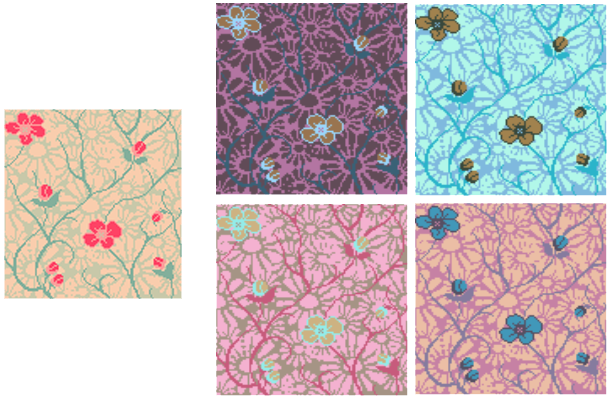
\includegraphics[width=0.7\columnwidth]{figs/badFlowers}
%\caption{(Left) An artist's coloring of a pattern. (Right) High-scoring colorings of the same pattern sampled from our model. When the colorings do not respect the semantics of the flower stems by making them biologically impossible colors, it becomes difficult to parse the resulting image as one depicting a cluster of flowers.}
%\label{fig:badFlowers}
%\end{figure}

% Future work: Templatizing images
This research opens up several interesting avenues for future work.
First, our experiments used patterns from COLOURlovers or renderings that can be easily coerced into the same format. What if any image found `in the wild' could serve as a recolorable pattern template? As a simple first approach, we could extract a color theme from the image, and then quantize the image using the theme's colors~\cite{SharonPaletteExtraction}. Such a simple approach is unlikely to perform well on complex images that use many distinct colors or color blending, however. Solving the problem in general requires further research.

% Future work: Patterns where color groups are unknown
Second, this work explores colorizing patterns of the `color-by-numbers' format, in which some pattern regions are constrained to take the same color. What if this assumption were relaxed, and the color groups in the pattern template are unknown? A system that supported this more general type of pattern template could operate on essentially any segmented image. This would require a more sophisticated model, as well as transdimensional inference techniques to generate recolorings with a variable number of color groups~\cite{YiTingLARJ}.

% Future work: Embed in real creative software
Finally, embedding automatic coloring suggestions into interactive creative software presents an exciting opportunity. A vector art program could continually generate suggestions in the background while its user works on a pattern; the user could view the suggestions at any time, potentially picking one to use as an `autocompletion' of her work-in-progress. These kinds of tools have the potential to drastically shift the way that artists and enthusiasts work with color on a daily basis. 